\documentclass{beamer}
\usetheme{Warsaw}
\usepackage[utf8]{inputenc}
\usepackage{hyperref}
\usepackage{xcolor}
\usepackage{multimedia}
\usepackage[linesnumbered,ruled,vlined]{algorithm2e}
\usepackage{physics}
\usepackage{float}
\usepackage{graphicx}
\usepackage{mathtools}
\usepackage{pgfpages}
\usepackage{dsfont}

\setbeameroption{show notes on second screen=right} % Speaker notes
\setbeamertemplate{footline}[frame number] 

% Give a slight yellow tint to the notes page
\setbeamertemplate{note page}{\pagecolor{yellow!5}\insertnote}\usepackage{palatino}

\newcommand{\snote}[1]{\textcolor{blue}{[*** Jamie : #1 ***]}}

\title[NSeS]{NISQ Algorithms for Separable Ground States}
%\subtitle{\url{https://github.com/ankith-mohan/SEP}}
\author{Ankith Mohan}
\institute{
    Department of Computer Science \\
    Virginia Tech
}
\date{4/5/2022}

\SetKwInput{KwInput}{Input}
\SetKwInput{KwOutput}{Output}

% Commands
\newcommand{\betamat}{\boldsymbol\beta}
\newcommand{\rhomat}{\boldsymbol\rho}
\newcommand{\sigmamat}{\boldsymbol\sigma}
\newcommand{\psivec}{\boldsymbol\psi}
\newcommand{\phivec}{\boldsymbol\phi}
\newcommand{\ivec}{\mathbf{i}}
\newcommand{\observable}{\boldsymbol\Pi}
\newcommand{\Amat}{\mathbf{A}}
\newcommand{\Cmat}{\mathbf{C}}
\newcommand{\Dmat}{\mathbf{D}}
\newcommand{\Emat}{\mathbf{E}}
\newcommand{\Pmat}{\mathbf{P}}
\newcommand{\Umat}{\mathbf{U}}
\newcommand{\Xmat}{\mathbf{X}}

\newcommand{\id}{\mathds{1}}
\newcommand{\Cspace}{\mathbb{C}}
\newcommand{\Sset}{\mathbb{S}}

\newcommand{\A}{\mathcal{A}}
\newcommand{\B}{\mathcal{B}}
\newcommand{\Hilbert}{\mathcal{H}}
\newcommand{\X}{\mathcal{X}}
\newcommand{\Y}{\mathcal{Y}}

\newcommand{\Pos}{\mathrm{Pos}}
\newcommand{\Sep}{\mathrm{Sep}}
\newcommand{\Herm}{\mathrm{Herm}}

\newcommand{\st}{\mathrm{s.t.}}

\begin{document}

\begin{frame}
	\titlepage
	\note[]{Thank everyone for being here.}
\end{frame}

\begin{frame}
	\begin{figure}
		\centering
		
\includegraphics[scale=0.4]{work-in-progress.jpg}
		\item[] Inner Approximations and NISQ Algorithms for the Separability Problem
		\item[] with Tobias Haug, Kishor Bharti and Jamie Sikora
		\note[item]{Start out by saying that this is still a work in progress in the sense that there are some measurement methods that have not yet been fully looked into.}
		\note[item]{This is part of the work in this paper which is also a work in progress}
	\end{figure}
\end{frame}

\AtBeginSection[]
{
  \begin{frame}{Outline}
    \tableofcontents[currentsection]
  \end{frame}
}

%\begin{frame} 
%\snote{Have an slide for each bound. $\alpha$ own slide and motivation. UPPER BOUNDS. $\beta$ for each bound. Symmetric extensions, mention how this set is larger then SEP, and thus $\beta \geq \alpha$. Mention realignment, and how this also relaxes $SEP$ (lower priority). Mention PPT and how this relaxes SEP. Summary slide: $\alpha \leq \min\{ \beta_1, \ldots, \}$.  
%        LOWER BOUNDS. Discuss see saw (in general) whole slide. OG see saw (whole slide). OG2. Randomized. $\alpha \geq \max \{ \gamma_1, \ldots \}$. 
%        SQUARE ROOT (special, new). Explain the "square root bound" ($\delta'$). Explain how they are/are not SDPs. Define $\delta$. 
%        SUMMARY. $\delta, \gamma, \ldots, \leq \alpha \leq \delta', \beta_1, \ldots$. Explain now that we want to test to see how good we are approximating $\alpha$.
%        New CHUNK: how to quantify goodness of bounds.
%        New Chunk: NISQ. Explain going from Big SEP problem to small SEP problem (why these bounds are useful).}
%\end{frame}

\section{NSS}
	\begin{frame}{NISQ SDP Solver}
		Hybrid quantum-classical algorithm to solve SDP.
		\begin{figure}
			\centering
			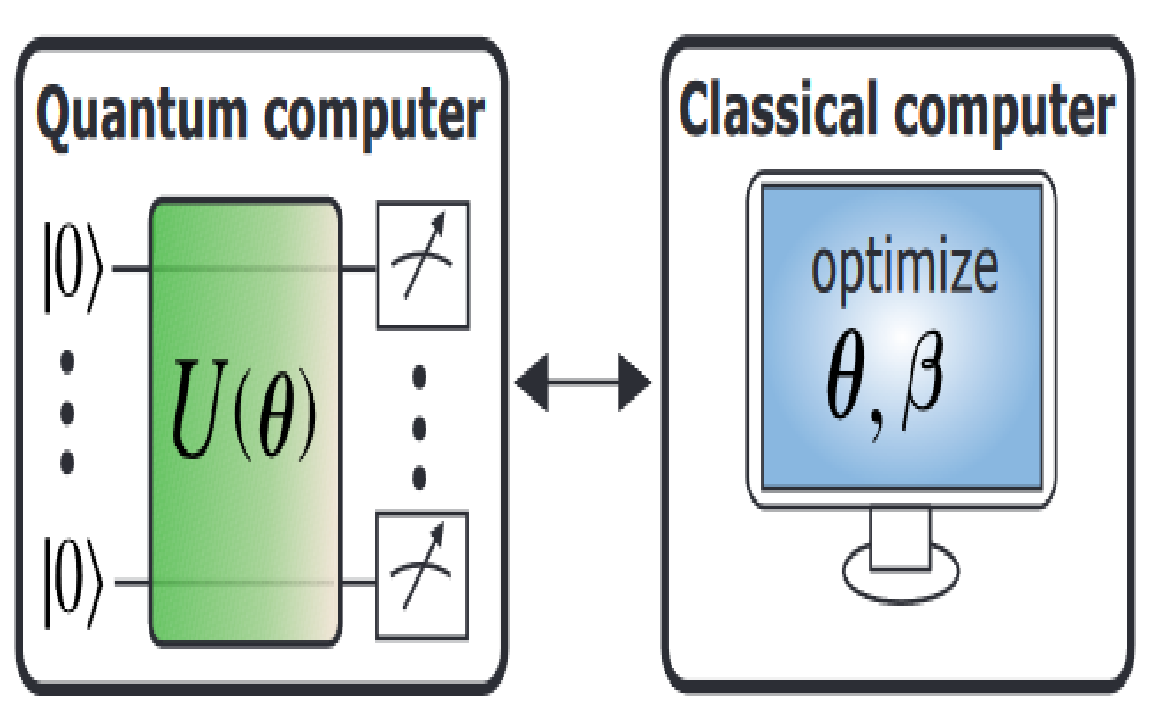
\includegraphics[height=75pt, width=250pt]{NSS.png}
		\end{figure}
		\begin{itemize}
			\item[] Quantum computer encodes an SDP. Only for estimating overlaps.
			\item[] Classical optimization routine is also an SDP with dimension given by the size of the ansatz space.
			\item[] No classical-quantum feedback loop.
		\end{itemize}
		
		\note[item]{Estimating overlaps can be done efficiently on current NISQ devices}
	\end{frame}

	\begin{frame}{Standard form primal SDP}
		\begin{equation}
			\begin{aligned}
				& \min \quad \langle \Cmat, \Xmat \rangle \nonumber \\
				& \hspace{5pt} \st \quad \langle \Amat_i, \Xmat \rangle = b_i,\ i = \{1, \dots, m\} \nonumber \\
				& \hspace{55pt} \Xmat \succcurlyeq 0 \nonumber
			\end{aligned}
		\end{equation}
		\vfill
		\begin{center}
			$\Cmat$ and $\Amat_i, \forall i$ are $n \times n$ Hermitian matrices.
		\end{center}
	\end{frame}

	\begin{frame}{NSS}
		3 distinct steps:
		\begin{enumerate}
			\item Ansatz selection
			\item Overlap measurement
			\item Post-processing
		\end{enumerate}
	\end{frame}

	\begin{frame}{Ansatz selection}
		\begin{enumerate}
			\item Set of $M$ quantum states $\Sset = \{\ket{\psivec_j} \in \Hilbert\}_j$ over a Hilbert space $\Hilbert$
			\item Hybrid density matrix ansatz
					$$
						\Xmat = \sum_{ij} \beta_{ij} \dyad{\psivec_i}{\psivec_j}
					$$
					where $\beta_{ij} \in \Cspace$
		\end{enumerate}
		\vfill
		$\Sset$ is prepared by a quantum computer. \\
		$\betamat$ is stored on a classical computer.
		\begin{block}{Lemma}
			$$
				\betamat \succcurlyeq 0 \implies \Xmat \succcurlyeq 0
			$$
		\end{block}
	\end{frame}
	
	\begin{frame}{SDP (Update 1)}
		\begin{equation}
			\begin{aligned}
				& \min \quad \langle \Cmat, \Xmat \rangle \nonumber \\
				& \hspace{5pt} \st \quad \langle \Amat_i, \Xmat \rangle = b_i,\ i = \{1, \dots, m\} \nonumber \\
				& \hspace{55pt} \Xmat \succcurlyeq 0 \hspace{185pt} \textcolor{orange}{\betamat \succcurlyeq 0} \nonumber
			\end{aligned}
		\end{equation}
		\vfill
		\begin{center}
			$\Cmat$ and $\Amat_i, \forall i$ are $n \times n$ Hermitian matrices.
		\end{center}
	\end{frame}

	\begin{frame}{Assumption}
		Assume $\Cmat$ and $\Amat_i, \forall i$ can be expressed as the sum of unitaries.
		\begin{align*}
			\Cmat &= \sum_k s_k \Umat_k \\
			\Amat_i &= \sum_l f_{il} \Umat_l^{(i)}
		\end{align*}
	\end{frame}
	
	\begin{frame}{Overlap measurement}
		Measure the following overlap on the quantum system
		\begin{align*}
			D_{ab} &= \sum_k s_k \bra{\psivec_b} \Umat_k \ket{\psivec_a}
		\end{align*}
	\end{frame}

	\begin{frame}{SDP (Update 2)}
		\begin{equation}
			\begin{aligned}
				& \min \quad \langle \Cmat, \Xmat \rangle \hspace{150pt} \textcolor{orange}{\min \quad \langle \betamat, \Dmat \rangle} \nonumber \\
				& \hspace{5pt} \st \quad \langle \Amat_i, \Xmat \rangle = b_i,\ i = \{1, \dots, m\} \nonumber \\
				& \hspace{55pt} \Xmat \succcurlyeq 0 \hspace{185pt} \textcolor{orange}{\betamat \succcurlyeq 0} \nonumber
			\end{aligned}
		\end{equation}
		\vfill
		\begin{center}
			$\Cmat$ and $\Amat_i, \forall i$ are $n \times n$ Hermitian matrices.
		\end{center}
	\end{frame}
	
	\begin{frame}{Overlap measurement}
		Measure the following overlap on the quantum system
		\begin{align*}
			D_{ab} &= \sum_k s_k \bra{\psivec_b} \Umat_k \ket{\psivec_a} \\
			E_{ab} &= \sum_l f_{il} \bra{\psivec_b} \Umat_l^{(i)} \ket{\psivec_a}
		\end{align*}
	\end{frame}
	
	\begin{frame}{Post-processing}
		\begin{equation}
			\begin{aligned}
				& \min \quad \langle \Cmat, \Xmat \rangle \hspace{150pt} \textcolor{orange}{\min \quad \langle \betamat, \Dmat \rangle} \nonumber \\
				& \hspace{5pt} \st \quad \langle \Amat_i, \Xmat \rangle = b_i,\ i = \{1, \dots, m\} \hspace{50pt}\textcolor{orange}{\st \quad \langle \betamat, \Emat^{(i)} \rangle = b_i} \nonumber \\
				& \hspace{55pt} \Xmat \succcurlyeq 0 \hspace{185pt} \textcolor{orange}{\betamat \succcurlyeq 0} \nonumber
			\end{aligned}
		\end{equation}
		\vfill
		\begin{center}
			$\Cmat$ and $\Amat_i, \forall i$ are $n \times n$ Hermitian matrices.
		\end{center}
	\end{frame}

	\begin{frame}{NISQ-friendly overlap measurement method (1)}
		Assumptions:
		\begin{enumerate}
			\item Unitaries $\Umat_k$ and $\Umat_l^{(i)}$ are Pauli strings $\Pmat = \bigotimes_{j=1}^N \sigmamat_j$ with $\sigmamat_j = \{\id, \sigmamat^{x}, \sigmamat^{y}, \sigmamat^{z}\}$.
					
					$\because$ Pauli strings form a complete basis, any matrix can be decomposed into a linear combination of Pauli strings.
					
			\item Ansatz space is generated by state $\ket{\psivec}$ and a set of $M$ different Pauli strings $\{\Pmat_1, \dots, \Pmat_M\}$ via $\Sset = \{\Pmat_j\ket{\psivec}\}_{j=1}^M$.
			
					$\implies$ Each overlap element can be expressed as a sum of expectation values of Pauli strings $\bra{\psivec}\Pmat_1 \Pmat_2 \Pmat_3\ket{\psivec} = a\bra{\psivec}\Pmat'\ket{\psivec}$, where $a \in \{+1, -1, +i, -i\}$.
					
					Measuring the expectation values of Pauli strings $\implies$ efficient calculation of the overlap elements.
		\end{enumerate}
		
		\note[item]{How do we actually measure the overlap?}
	\end{frame}
	
	\begin{frame}{NISQ-friendly overlap measurement method (2)}
		\begin{itemize}
			\item On NISQ computers, perform single-qubit rotations into the eigenbasis of the Pauli operator and sample in the computational basis.
			\item For $\Sset = \{\Pmat_j\ket{\psivec}\}_{j=1}^M$ we are only required to prepare the reference state $\ket{\psivec}$.
			\item Other states are related to the reference state via single layer Pauli unitaries.
			\item $\therefore$ we only have to sample $\ket{\psivec}$ in a set of Pauli rotated basis elements.
		\end{itemize}
	\end{frame}

\section{NSeS}
	\begin{frame}{Problem Statement}
		\begin{itemize}
			\item[] Given $\rhomat \in \Pos(\A \otimes \B)$, we want to determine whether $\rhomat$ is \emph{separable} or \emph{entangled}?
			\item[] Formally, we define 
			$$
				\Sep(\X : \Y) = \left \{ \sum_{i=1}^k p_{i} \dyad{\psivec_i} \otimes \dyad{\phivec_i} : \sum_{i=1}^k p_{i} = 1, p_i \ge 0\ \forall\ i \right \}
			$$
			\begin{center}
				$\rhomat \in \Sep(\A : \B)?$
			\end{center}
			\pause
			\item[] Equivalently: Given $\observable \in \{\Pos(\A \otimes \B), \Herm(\A \otimes \B)\}$, we want to compute:
			$$
				\alpha = \sup\limits_{\rhomat \in \Sep} \langle \rhomat, \observable \rangle
			$$
			\item[] This is known to be a NP-hard problem~\cite{gurvitz2003}
		\end{itemize}
        
		\note[item]{bipartite density matrix $\rhomat$ -- entangled?}
		\note[item]{set of separable states as the convex combination of tensor product of pure states}
		\note[item]{so we ask does $\rhomat$ belong to this set?}
		\note[item]{This is equivalent to asking the following optimization problem: given a PSD or Herm operator, what is the density matrix that maximizes this HSIP?}
	\end{frame}

	\begin{frame}{Ansatz selection}
		\begin{itemize}
			\item[] $\Sset_A = \{\ket{\psivec_i}\}_{i=1}^N \in \A$
			\item[] $\Sset_B = \{\ket{\phivec_j}\}_{j=1}^M \in \B$
			\item[] Hybrid density matrix ansatz
						$$
							\Xmat = \sum_{ijkl} \beta_{ijkl} \dyad{\psivec_i}{\psivec_j} \otimes \dyad{\phivec_k}{\phivec_l}
						$$
						where $\beta_{ijkl} \in \Cspace$
		\end{itemize}
	\end{frame}
        
	\begin{frame}{Original Problem}
		\begin{equation}
			\begin{aligned}
				& \sup \quad \langle \Xmat, \observable \rangle \nonumber \\
				& \hspace{5pt} \st \quad \Tr(\Xmat) = 1 \nonumber \\
				& \hspace{50pt} \Xmat \in \Sep(\A : \B) \nonumber
			\end{aligned}
		\end{equation}
	\end{frame}

	\begin{frame}{Lemma}
		$$
			\betamat \in \Herm(\A' \otimes \B')
		$$
		where
		\begin{align*}
			\dim(\A') &<< \dim(\A), \\
			\dim(\B') &<< \dim(\B)
		\end{align*}
		\pause
		\begin{block}{Lemma}
			$$
				\betamat \in \Sep(\A' \otimes \B') \implies \Xmat \in \Sep(\A \otimes \B)
			$$
		\end{block}
	\end{frame}

	\begin{frame}{Problem (Update 1)}
		\begin{equation}
			\begin{aligned}
				& \sup \quad \langle \Xmat, \observable \rangle \nonumber \\
				& \hspace{5pt} \st \quad \Tr(\Xmat) = 1 \nonumber \\
				& \hspace{50pt} \Xmat \in \Sep(\A : \B) \hspace{100pt} \textcolor{orange}{\betamat \in \Sep(\A' : \B')} \nonumber
			\end{aligned}
		\end{equation}
	\end{frame}

	\begin{frame}{Overlap measurement}
		Assume $\observable$ can be expressed as a sum of unitaries
		$$
			\observable = \sum_x c_x \Umat_x
		$$
		Measure the following overlaps:
		\begin{align*}
			D_{ijkl} &= \sum_x c_x \ket{\psivec_j} \ket{\phivec_l} \Umat_x \ket{\psivec_i} \ket{\psivec_k} \\
			E_{ijkl} &= \braket{\psivec_j}{\psivec_i} \braket{\phivec_l}{\phivec_k}
		\end{align*}
	\end{frame}
        
	\begin{frame}{Post-processing}
		\begin{equation}
			\begin{aligned}
				& \sup \quad \langle \Xmat, \observable \rangle \hspace{150pt} \textcolor{orange}{\sup \quad \langle \betamat, \Dmat \rangle} \nonumber \\
				& \hspace{5pt} \st \quad \Tr(\Xmat) = 1 \hspace{130pt} \textcolor{orange}{\st \quad \langle \betamat, \Emat \rangle = 1} \nonumber \\
				& \hspace{55pt} \Xmat \in \Sep(\A : \B) \hspace{125pt} \textcolor{orange}{\betamat \in \Sep(\A' : \B')} \nonumber
			\end{aligned}
		\end{equation}
	\end{frame}

\section{Quantification}
	\begin{frame}{Upper bounds}
		\begin{itemize}
			\item $\beta_{PPT}$: PPT criterion~\cite{horodecki1996PPT},~\cite{peres1996PPT}
			\item $\beta_r$: Realignment criterion~\cite{chen2003realignment}
			\item $\{ \beta_1, \dots, \beta_k \}$: Symmetric Extensions~\cite{chen2014SymExt}
			\item $\{ \beta'_1, \dots, \beta'_k \}$: Bosonic Extensions~\cite{li2019BosExt}
		\end{itemize}
	\end{frame}

	\begin{frame}{See-saw}
		\begin{algorithm}[H]
			\KwInput{$\sigmamat_A \in \Pos(\A),\ \observable$} 
			\KwOutput{$\gamma$}
			\Repeat{convergence or maximum number of iterations}{
				$\sigmamat_B: \sup \limits_{\sigmamat_B \in \Pos(\B)} \langle \sigmamat_A \otimes \sigmamat_B, \observable \rangle$ \\
				$\sigmamat_A: \sup \limits_{\sigmamat_A \in \Pos(\A)} \langle \sigmamat_A \otimes \sigmamat_B, \observable \rangle$
			}
			$\gamma = \langle \sigmamat_A \otimes \sigmamat_B, \observable \rangle$
			\caption{see-saw}
		\end{algorithm}
	\end{frame}
	
	\begin{frame}{Lower-bounds}
		\begin{align*}
			\gamma_{MM} &= \mbox{see-saw} \left( \frac{1}{\dim\A}\,\id, \observable \right) \\
			\gamma_{US} &= \mbox{see-saw} \left( \frac{1}{\dim\A}\,\sum_i \dyad{\ivec}, \observable \right) \\
			\gamma_{rand} &= \mbox{see-saw} \left( \mbox{random vector}, \observable \right) \mbox{ for 100 points}
		\end{align*}
	\end{frame}

	\begin{frame}{Summary}
		$$
            \{ \gamma_{MM}, \gamma_{US}, \gamma_{rand} \} \le \alpha \le \{ \beta_{PPT}, \beta_r, \beta_1, \dots, \beta_k, \beta'_1, \dots, \beta'_k \}
        $$
	\end{frame}

	\begin{frame}{Quantification}
		\begin{itemize}
			\item[] How well are we really approximating $\alpha$?
			\item[] Define ``Tightness of Bound" (TOB) as
						$$
							ToB = \beta - \gamma
						$$
						where
						\item[] 
							$$
								\beta = \min \{ \beta_{PPT}, \beta_r, \beta_1, \dots, \beta_k, \beta'_1, \dots, \beta'_k \}
                				$$
                			\item[]
                				$$
                    				\gamma = \max \{ \gamma_{MM}, \gamma_{US}, \gamma_{rand} \}
                				$$
		\end{itemize}
	\end{frame}

\section{Results}
	\begin{frame}{Results}
		\url{https://ankith-mohan.shinyapps.io/SEP_app}
	\end{frame}
            
\bibliographystyle{apalike}
\bibliography{NSeS}
    
\end{document}
